% !TEX root = ./chemistry.tex

\chapter{Module 5 \; Equilibrium and Acid Reactions}

\section{Le Chatelier's Principle} \label{29/10/2024-31/10/2024}
	"If a system at equilibrium is subject to a change in conditions, then the system will behave in such a way so as to partially counteract the imposed change"

	Haber process:

	\subsection{Effect of Concentration}
		\begin{equation}
			\ce{N2\gas{} + 3H2\gas{} <=> 2NH3\gas{} \quad \enthalpy{-92.5}}
		\end{equation}
		

	\subsection{Effect of Pressure}
	\subsection{Effect of Partial Pressure}
	\subsection{Effect of Volume}
		Decreasing the volume will increase the pressure. (Boyle's Law) This increases the collision rate between the reactants and favours the forward reaction.

	\subsection{Effect of Temperature}
		asd
	
	\subsection{Summary}
		To use Le Chatelier's principle to predict the outcome of a change in conditions, you need to consider the following points.
		\begin{enumerate}
			\item What change is imposed?
			\item What is the opposite of the change?
			\item Which reaction direction is favoured - the forward or reverse?
			\item Does equilibrium shift to the left or right?
			\item What happens to the concentrations of each aqueous substance or gas?
		\end{enumerate}

	\begin{figure}[H]
		\centering
		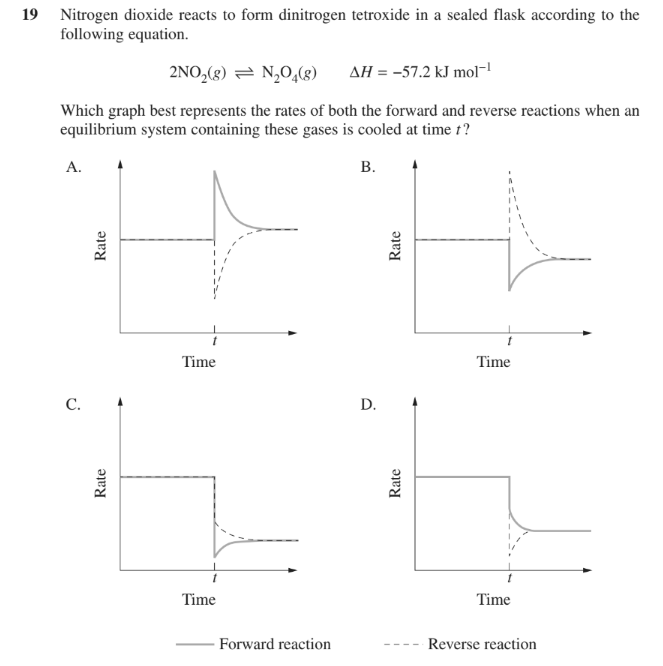
\includegraphics{Le Chatelier's example problem}
	\end{figure}

	\textbf{D} When temperature decreases, the rates of both forward and backward reactions will decrease regardless of which way the endothermic or exothermic reaction goes. (A and B can be eliminated)

	This is because all the particles in the system lose kinetic energy, decreasing the rate of collisions hence, decreasing the rate of reaction.
	
	However, since there is a decrease in temperature the exothermic reaction will be favoured in order to counteract the change. In this case, the forward reaction being exothermic is affected less by the drop in temperature as shown in D.

\pagebreak
\section{Practical Investigation 2.3 - Effect of changes to concentration on equilibrium} \label{31/10/2024}

	Aim: To observe the effect of a change in concentration on a system at equilibrium

	\subsection{Materials}
		\begin{itemize}
			\item 2 mL of 0.1 molL$^{-1}$ iron(III) chloride solution
			\item 2 mL of 0.1 molL$^{-1}$ ammonium thiocyanate solution
			\item 1 mL of 0.1 molL$^{-1}$ calcium fluoride solution
			\item 20 mL distilled water
			\item 2x 10 mL measuring cylinders
			\item 25 mL measuring cylinder
			\item 4 test tubes
			\item Test-tube rack
			\item 4 small labels
			\item Disposable 1 mL droppers
			\item Waste bottle
			\item Digital camera
			\item Safety glasses
		\end{itemize}

	\subsection{Risk Assessment}
		\begin{table}[htbp]
			\centering
			\begin{tabular}{l|l}
				\hline
				Hazard & Precaution \\ \hline
				Chemicals may splash onto skin or eyes & Wear safety glasses and wash hands  \\
				Chemicals may harm aquatic life & Place in inorganic waste container \\
			\end{tabular}
		\end{table}

	\subsection{Method}
		\begin{enumerate}
			\item Pour 1 mL of iron(III) chloride solution into a 10 mL measuring cylinder.
			\item Pour 1 mL of ammonium thiocyanate into another 10 mL measuring cylinder.
			\item Pour both solutions into the 25 mL measuring cylinder.
			\item Add 18 mL of distilled water to the 25 mL measuring cylinder so that the total volume is 20 mL.
			\item Label four test tubes A, B, C and D.
			\item Pour equal volumes of the solution in the 25 mL measuring cylinder into each of the test tubes.
			\item Retain test tube A as the reference solution.
			\item Add 1 mL of iron(III) chloride to test tube B.
			\item Take a photo to record observations for test tube B relative to test tube A.
			\item Add 1 mL of ammonium thiocyanate to test tube C.
			\item Take a photo to record observations for test tube C relative to test tube A.
			\item Add 1 mL of calcium fluoride to test tube D. (Note: This reacts with the iron(III) ion so there is less iron(III) available to react with the thiocyanate ion.)
			\item Take a photo to record observations for test tube D relative to test tube A
		\end{enumerate}

	\subsection{Results}
		\begin{figure}[H]
			\centering
			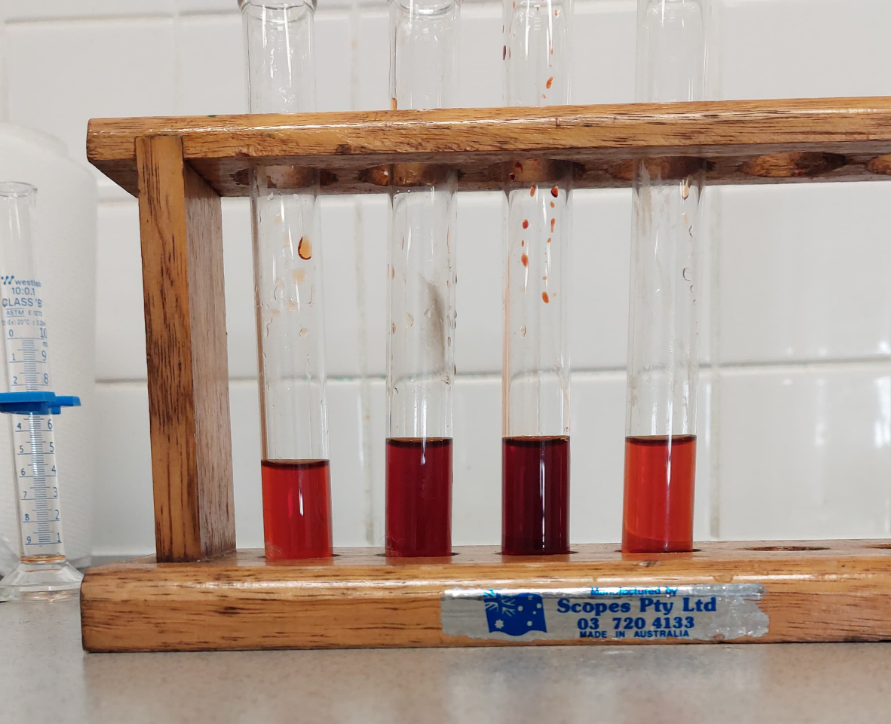
\includegraphics{Practical Investigation 2.3 - Results.png}
			\caption{Test tubes A, B, C, D}
		\end{figure}

	\subsection{Discussion}
		\textbf{Explain each colour change in terms of collision theory.}

		The test tube B was darker in colour in comparison to test tube A. The increase in moles of reactants allows more successful collisions to occur, increasing the amount of product. The same principle applies to test tube C.

		Test tube D was lighter in colour compared to A, due to the calcium fluoride reacting with the iron (III) chloride 

	\subsection{Conclusion}
		\textbf{Use Le Chatelier's principle to explain what happened in test tubes B, C and D.}

		Test tube B was darker due to the increase in concentration of the reactant iron (III) chloride causes a shift of the equilibrium towards the products due Le Chatelier's principle
		
		Test tube C was darker due to the increase in concentration of the reactant ammonium thiocyanate causes a shift of the equilibrium towards the products due Le Chatelier's principle

		Test tube D was lighter because the calcium fluoride reacted with the iron (III) chloride, lowering the overall concentration of iron (III) chloride. This reduced the amount of reactants available, making the reverse reaction more favourable by Le Chatelier's principle.

\section{Calculating the Equilibrium Constant} \label{5/11/2024}
	The equilibrium constant can be used to predict the direction of chemical reactions

	$$K_{eq} = \frac{[products]}{[reactants]}$$
	For reaction:
	$$\ce{aA + bB <=> cC + dD}$$
	the equilibrium expression is:
	$$K_{eq}=\frac{[C]^{c}[D]^{d}}{[A]^a[B]^b}$$

	The concentration of each chemical species is raised to the power of the number of moles of that species indicated in the chemical equation. (Eg. there are $d$ moles of species $D$, hence in the equilibrium expression the concentration of species $D$ is raised to the power of $d$, written as $[D]^d$)

	\begin{itemize}
		\item The value for the equilibrium constant only takes into account the concentration of substances where the concentration can vary
		\item Solutions and gases can vary in concentration or partial pressure hence are included in $K_{eq}$
		\item Solids and pure liquids are NOT included eg. $\ce{H_2O}$ isn't required when calculating
	\end{itemize}

	\subsection{Reaction Quotient ($Q$)}
		$$Q=\frac{[C]^{c}[D]^{d}}{[A]^a[B]^b}$$
		Has the same formula as $K_{eq}$, however applies to any stage of a reaction
		
	\subsection{Equilibrium Constant}
		\begin{itemize}
			\item Comparing $Q$ to $K_{eq}$ predicts which way the equilibrium will shift
			\item $K_{eq}$ is where the equilibrium lies
			\item A large $K_{eq}$ means that there are more products than reactants; ie. equilibrium lies towards completion
			\item If $K_{eq}$ is close to one, both reactans and products are plentiful at equilibrium
		\end{itemize}
		\textbf{Example} Let $Q=2.1$, $K_{eq}=0.315$, $\therefore$ products$>$reactants.

	\subsection{Calculating the equilibrium expression}
		Consider the reaction between hydrogen and iodine producing hydrogen iodide:
		$$\ce{H_{2}\gas{} + I_{2}\gas{} <=> 2HI\gas}$$

\section{ICE Tables} \label{6/11/2024}
	\begin{table}[htbp]
		\centering
		\begin{tabular}{|l|l|l|l|}
			\hline
			 & [A] & [B] & [C] \\ \hline
			Initial concentration &  &  &  \\
			Change in concentration &  &  &  \\
			Equilibrium concentration &  &  &  \\ \hline
		\end{tabular}
	\end{table}

	$$\Delta c = c_{eq}- c_{u}$$

	Eg. $\ce{A + B <=> C + D}$

	\begin{table}[htbp]
		\centering
		\begin{tabular}{lllll}
			\hline
			 & [A] & [B] & [C] & [D]  \\ \hline
			Initial concentration 		& 0.6 & 0.6 & 0 & 0 \\
			Change in concentration 	& -0.5 & -0.5 & +0.5 & +0.5 \\
			Equilibrium concentration 	& 0.1 & 0.1 & 0.5 & 0.5 \\ \hline
		\end{tabular}
	\end{table}

\newpage
	Eg. $\ce{2X \gas{} <=> 3Y \gas{} + 4Z \gas{}}$

	A sample consisting of 0.500 mol of X is placed into a system with a volume of 0.750 liters. \\
	At equilibrium, the amount of sample X is known to be 0.350 mol.

	\begin{table}[htbp]
		\centering
		\begin{tabular}{cccc}
			\hline
			 & X & Y & Z \\ \hline
			I 		& 0.5 & 0 & 0 \\
			C 		&  &  & \\
			E 		& 0.35 &  &  \\ \hline
		\end{tabular}
	\end{table}

	\begin{table}[htbp]
		\centering
		\begin{tabular}{cccc}
			\hline
			 	& X & Y & Z \\ \hline
			I 		& 0.5 & 0 & 0 \\
			C 		& -0.15 & -0.225 & +0.3 \\
			E 		& 0.35 & 0.225 & 0.3 \\ \hline
		\end{tabular}
	\end{table}

	\begin{align*}
		[X] &= \frac{0.35}{0.75} = 0.467 \\
		[Y] &= \frac{0.225}{0.75} = 0.3 \\
		[Z] &= \frac{0.3}{0.75} = 0.4
	\end{align*}
	
\section{Effect of Temperature on $K_{eq}$} \label{8/11/2024}
	Although other factors may affect equilibrium, $K_{eq}$ is only affected by temperature.
	Changing concentration, pressure, or volume will change the concentrations and therefore adjust the reaction point, however the reaction will still equalise to achieve the same $K_{eq}$

	\begin{itemize}
		\item For a particular reaction, $K_{eq}$ is constant at a given temperature
		\item Temperature changes the ratio of products and reactants, hence changing $K_{eq}$
		\item For $\ce{N2O2 \gas{} <=> 2NO2 \gas{}}$, temperature increases the $K_{eq}$ value and favours the formation of products. The forward reaction is endothermic
	\end{itemize}

	\subsection{Example Question}
		Nitric oxide gas ($\ce{NO}$) can be produced from the direct combination of nitrogen gas and oxygen gas in a reversible reaction.
		\begin{enumerate}
			\item \textbf{Write a balanced chemical equation for this reaction (1 mark)}
				\subitem $\ce{N2 \gas{} + O2 \gas{} <=> 2NO \gas{}}$
			\item \textbf{Explain, using collision theory, how an increase in temperature would affect the value for $K_{eq}$ for this system. Refer to the diagram in your answer.}
				\subitem An increase in temperature would favour the forward reaction, hence $K_{eq}$ will increase. More energy allows more collisions to occur
		\end{enumerate}
	
		\begin{align*}
			K_{eq} &= \frac{[p_1][p_2]}{[r_1][r_2]} \\
			1 &= \frac{[1][1]}{[1][1]} \\
		\end{align*}
		\centering If $p_2$ decreases to $[0.5]$, favouring the forward reaction
		\begin{align*}
			&= \frac{[1.15][0.65]}{[0.85][0.85]} \\
			&=K_{eq}
		\end{align*}